\chapter{Einleitung}\label{ch:einleitung}
\glqq I recently predicted the last mainframe will be unplugged on March 15, 1996\grqq\footnote{\cite{Alsop.1993}} - ein in der Großrechner-Welt bekannt gewordenes Zitat.
Es handelt sich um eine 1993 getroffene Vorhersage, nämlich dass der letzte Mainframe, auch Großrechner genannt, am 15 März 1996 abgeschaltet werden wird.
Wieso wird sich im Jahre 2020 dennoch mit dieser Technologie beschäftigt? 
Und was genau ist ein Großrechner?

In einem Satz ist ein Großrechner\footnote{Beschreibung im Absatz \ref{sec:mainframe} zu finden} ein leistungsstarkes, zentralisiertes Serversystem.
In dieser Arbeit wird nur auf Mainframes aus dem Hause von IBM eingegangen.
Damit ist auch der Technologiestack festgelegt.
Das verwendete Betriebssystem ist z/OS, darauf werden Middleware Produkte wie CICS\footnote{Anwendungsserver, CICS Beschreibung Absatz \ref{cics}}, das Datenbanksystem Db2\footnote{ Beschreibung Absatz \ref{sssec:db2}} sowie die Messaging Lösung \glqq IBM MQ\grqq{}\footnote{Beschreibung im Absatz \ref{sec:mq} zu finden} betrieben.
Als Programmiersprachen werden COBOL, IBM Assembler, C und C++ verwendet, sowie seit ca. 23 Jahren Java.\footnote{\cite{Steegmans.2003}}.

Der IBM Mainframe hat eine lange Geschichte.
Vor mehr als fünfzig Jahren wurde der allererste Großrechner, der sog.(Kommentar: Bezeichnung such ich noch raus) vorgestellt.
Bis in die 90iger Jahre spielte der IBM Mainframe eine Hauptrolle auf dem Computermarkt, dann gewannen zunehmend verteilte Client-Server-Systeme an Bedeutung.\footnote{\cite{Ceruzzi.2003}}
Seitdem gilt der Mainframe bereits als \glqq  legacy\grqq{}- veraltet -.
Im Jahre 2020 ist der größte Konkurrent für den Mainframe die Cloud.
Laut einer Vorhersage aus dem Jahr 2018\footnote{Statistik im Anhang \ref{app:itworkload}} soll circa 79 Prozent des weltweiten Workloads in einer Cloud verarbeitet werden.

Wieso also wird sich mit der Mainframe Technologie noch beschäftigt? - Eine Antwort: Der Mainframe wird weltweit genutzt.
So verarbeiten Großrechner auch heutzutage weltweit circa 1,2 Millionen CICS Transaktionen pro Sekunde.\footnote{\cite{IBM.2019}}
Im Vergleich hierzu werden 63.000 Google Suchanfragen pro Sekunde abgesetzt. \footnote{\cite{Sullivan.2016}}

Aus der Kombination von hohem Workload, dem proprietären, IBM-abhängigen Technologiestack und dem Ruf eines veralteten Systems entstehen jedoch zunehmend Risiken.
Es wird immer schwieriger Nachwuchs in diesem Bereich zu finden.
Zum einem, da es kaum noch an Universitäten gelehrt wird.
Die Seite des Hochschulkomasses\footnote{\cite{internetagenturKolnFrankfurtsunzinetTYPO3Programmmierung.}} liefert sogar weder für \glqq Mainframe\grqq{} noch für \glqq Großrechner\grqq{} einen Treffer.
Zum anderen ist der demographische Faktor, der Wissensträger nicht zu vernachlässigen.
Ein weiteres Problem ist, dass eine Firma, die einen IBM Großrechner mit z/OS betreibt, von dem oben genannten proprietären Technologiestack abhängig ist, dass heißt es entsteht eine starke Herstellerabhängigkeit.

Offensichtlich betreiben dennoch einige Firmen einen IBM Großrechner.
Darunter zählen hauptsächlich Banken, das Gesundheitswesen, Versicherungen, Fluggesellschaften usw.
Der gemeinsame Nenner dieser Unternehmen ist, dass sich über die Jahre und Jahrzehnte enorme Investitionen auf dem Mainframe angesammelt haben.
Die entstandenen Kernsysteme haben hohe Anforderungen an Massendatenverarbeitung, Sicherheitsstandards und Hochverfügbarkeit.
All diese Punkte sprechen nach wie vor für die Nutzung eines Großrechners, auch bei der DATEV eG.
\cite{IBM.2014}

Die DATEV eG wurde am 14.02.1966 von 65 Steuerbevollmächtigten gegründet.
Sie verfolgten mit der Gründung das Ziel, Buchführungsaufgaben mit Hilfe der neu aufkommenden EDV zu bewältigen.
Aufgrund hohen Mitgliederwachstums wurde hierfür bereits 1969 in einen firmeneigenen IBM-Großrechner investiert.\cite{DATEVeG.2017}
Heute umfasst das Leistungsspektrum der DATEV eG unter anderen das Rechnungswesen, Personalwirtschaft, Consulting, IT-Sicherheit, Weiterbildung.
Ein nicht unbeträchtlicher Teil dieser betriebswirtschaftlichen Anwendungen läuft bis heute auf einem IBM Großrechner im DATEV Rechenzentrum.
So werden pro Tag circa 150.000 Batch Jobs\footnote{Beschreibung in Absatz \ref{ssec:job}} und circa 90 Millionen CICS-Transaktionen verarbeitet.
Diese Last wird von circa 14.000 aktiven Modulen erzeugt.
Wie in der Abbildung \ref{fig:Programmiersprachen} zu sehen ist, ist COBOL mit circa 46\% Prozent die am häufigsten verwendete Programmiersprache am Großrechner bei der DATEV eG.
Durch diese Module werden unter anderem im Monat circa 11 Millionen Lohnabrechnungen erstellt und circa eine Millionen Umsatzsteuer-Voranmeldungen durchgeführt.

\begin{figure}
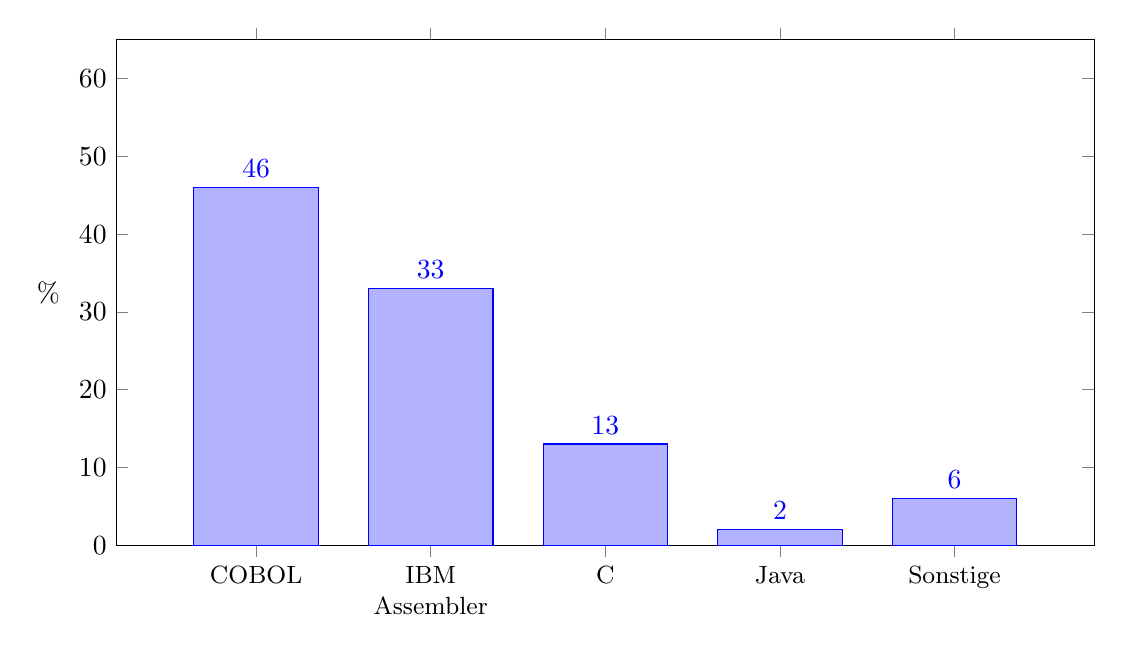
\begin{tikzpicture}
\begin{axis}[
             width=14cm,
             height=8cm,
             symbolic x coords={COBOL,IBM Assembler,C,Java, Sonstige},
             x tick label style={font=\small,text width=1.7cm,align=center},
             xtick=data,
             nodes near coords,
      	  nodes near coords align={vertical}, 
             ymin=0,
             ymax=65,
             ylabel=\%,
             ylabel style={rotate=-90},
             ybar,
             enlarge x limits=.2,
             bar width=45pt,
             ]
\addplot coordinates{(COBOL,46) (IBM Assembler,33) (C,13) (Java,2) (Sonstige,6)};
\end{axis}
\end{tikzpicture}
\centering
\caption{Anteil der verwendeten Programmiersprachen auf dem Mainframe bei DATEV eG in Prozent}
\label{fig:Programmiersprachen}
\end{figure}

Ich persönlich habe eine Ausbildung zum Fachinformatiker der Anwendungsentwicklung im Großrechnerbereich bei der DATEV eG abgeschlossen und parallel dazu ein Studium der Informatik begonnen.
Während dieser Ausbildung lernte ich unter anderem die Entwicklungsprozesse für den Mainframe kennen.
Kurz bevor ich die Ausbildung begonnen hatte, wurde eine auf Eclipse basierende Entwicklungsumgebung für COBOL und IBM Assembler in der DATEV eG flächendeckend eingeführt.
Zuvor wurde mit Hilfe der in Abbildung \ref{fig:3270} gezeigten Oberfläche, dem sog. ISPF gearbeitet.
Diese stellte z.B. nur ein Syntaxhighlighting zur Verfügung.

\begin{figure}[h]
\centering
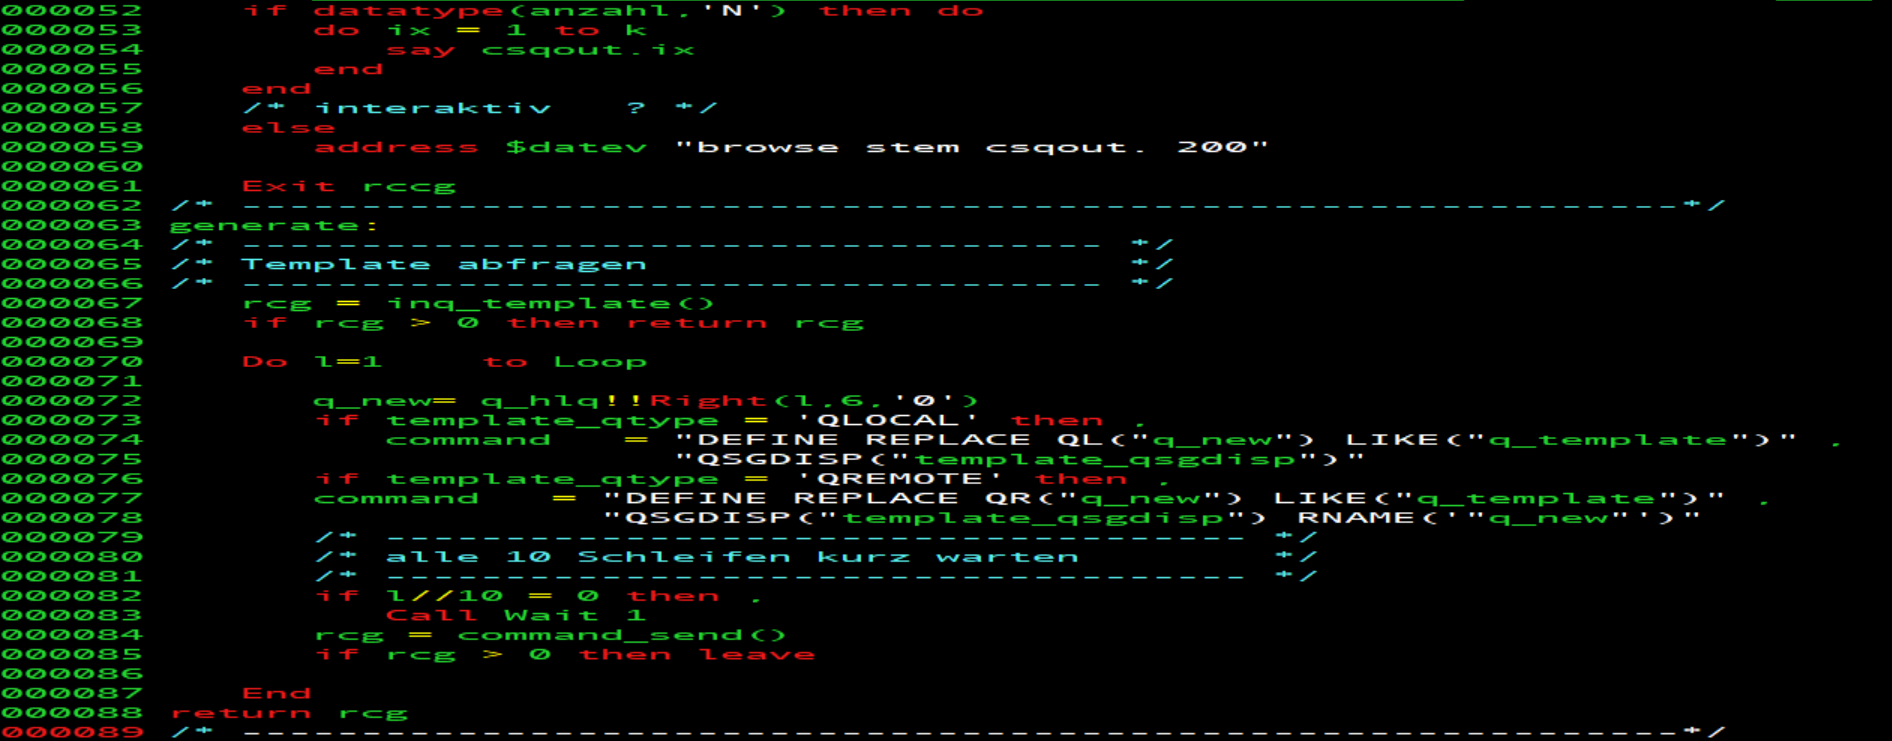
\includegraphics[width=\textwidth]{figures/rexxintso.png}
\caption{Auszug aus einem REXX Skript in der ISPF Oberfläche}
\label{fig:3270}
\end{figure}

Kurz vor Abschluss meiner Ausbildung wurde git, das Standard-Sourcverwaltung für verteilte Systeme und Cloud Entwicklung, auch für COBOL und IBM Assembler Sourcen eingeführt.
Dadurch wurde ein bis dato verwendetes eigenentwickeltes Tool für die Sourceverwaltung der z/OS Sourcen abgelöst.
Jedoch wurde damit zwar das Tooling modernisiert, jedoch nicht der Entwicklungsprozess selbst.
Entwickelt wird in einer sogenannten \glqq Entwicklungsstage\grqq{}\footnote{Beschreibung der Stages in Absatz \ref{sec:sysplex}}. 
So teilen sich zumindest die Entwickler einer Anwendung die gleiche Test-CICS/Db2/MQ Ressourcen.
Das heißt auch, dass eine Parallelentwicklung an unterschiedlichen Features nur mit viel Abstimmungs-Aufwand und Absprachen innerhalb eines Entwicklungsteams, teilweise auch abteilungsübergreifend, möglich ist.
Die Verantwortung der Systemressourcen, unter anderem auch der Test Ressourcen, liegt bei extra dafür entstandenen Administratorenteams.
Werden Änderungen an bestehenden Ressourcen durchgeführt oder werden neue Systemumgebungen benötigt, entsteht weiterer Abstimmungs-Aufwand und weitere Absprachen.
Dadurch wird der Prozess fehleranfällig und langsam.
In der Cloud Entwicklung sind dagegen moderne Prozesse, bei denen eine automatisierte Bereitstellung von Systemumgebungen, zum Beipiel einer Datenbank, über einen \glqq Marktplatz\grqq, Standard. 

Moderne Entwicklungsprozesse durfte ich nach dem Abschluss meiner Ausbildung in einem \glqq Cloud Native\grqq-Projekt selbst erleben.
Hier hatte jeder Entwickler seine eigene Testumgebung und konnte isoliert und ungestört von seinen Kollegen, ein neues Feature testen.
Die Datenbank konnte per Knopfdruck bereitgestellt werden, ganze Laufzeitumgebungen konnten auf diese Weise erzeugt werden.
Solche Prozesse unterstützen die bei DATEV e.G. eingesetzte agile Softwareentwicklung, und von den zuständigen Abteilungen, die sich mit der Modernisierung von z/OS Anwendungen und -prozessen beschäftigen,  kam die Frage auf, ob es möglich wäre, solche Mechanismen auch für legacy z/OS Anwendungen aufbauen zu können.
In Zusammenarbeit mit dem Bereich IT-Services und Technologiestrategie ergab sich damit das Thema für diese Arbeit, in der folgende Fragen beantwortet und bewertet werden sollen.

Ist es generell technisch möglich mit dem \glqq IBM Cloud Provisioning and Management for z/OS\grqq-Toolkit Laufzeitumgebungen automatisiert bereitzustellen?
Wird dadurch der aktuelle Bereitstellungsprozess schneller und auch sicherer?
Erzeugt die Nutzung einen Mehrwert bei den Stakeholdern, also den Entwicklerteams und den Administratorenteams?

Um diese Fragen zu beantworten wird die Provisionierung einer z/OS Laufzeitumgebung für eine spezielle Anwendung untersucht.
Die Anwendung sollte ein CICS als Anwendungsserver, eine Db2 Datenbank und IBM MQ als Messaginglösung benötigen, um für diese 3 Haupt-Technologien (Middleware-Komponenten) eine Aussage treffen zu können.
Die genaue Vorgehensweise wird im Kapitel \ref{ch:vorgehensweise} beschrieben.